\documentclass[10pt,hyperref={CJKbookmarks=true},xcolor=dvipsnames,aspectratio=169]{beamer}
\usetheme[navigation]{UMONS}
\usepackage[utf8]{inputenc}
\usepackage{verbatim}
\usepackage{ctex}

\title[国际经济学]{国际经济学}
\subtitle{劳动力的跨国流动:移民模型}
\author{鲁晓东}
\institute[]{%
	岭南学院\hspace{2em}中山大学
	\\[4ex]
	
\includegraphics[height=8ex]{fig/lingnanlogo}\hspace{2em}%
	
\includegraphics[height=8.5ex]{fig/sysu}
}
%------------section前展示一页----------
\AtBeginSection[] {     
	\begin{frame}        
	\tableofcontents[currentsection,hideallsubsections]    
\end{frame} 
}

%-------------subsection也展示一下----------
\AtBeginSubsection[]{

\frame<beamer>{ 
	
	\frametitle{Outline}   
	
	\tableofcontents[currentsection,currentsubsection] 
	
}

}
%---------------------------

%-----------一段一闪现-------
%\beamerdefaultoverlayspecification{<+->}
%这个功能基本不用

\begin{document}
\maketitle


\begin{frame}
\frametitle{提纲}
\tableofcontents
\end{frame}				%生成提纲页

%-----------正文开始----------------------



\section{Motivation}
\begin{frame}{Memories of Mariel}

\begin{columns}[onlytextwidth]
	\begin{column}{0.4\textwidth}
		\begin{itemize}
			\item 面对日益增强的不同政见、住房和工作短缺以及急剧衰退的经济,古巴总理菲德尔•卡斯特罗于1980年4月4日从在哈瓦那的秘鲁大使馆撤走了卫队。……在卫队撤走后不到48小时,大群的古巴人涌入了郁郁葱葱的秘鲁大使馆庭院,要求避难…… 4月中旬,卡特总统签发了一份总统备忘录允许最多3 500名难民在美国避难……但当4月21日难民开始抵达佛罗里达海滩时,卡特政府被惊呆了——难民数量最终达到了125000人。
			 \item Mariel移民会不会压低迈阿密其他工人的工资?
		\end{itemize}

		
	\end{column}
	\begin{column}{0.6\textwidth}
		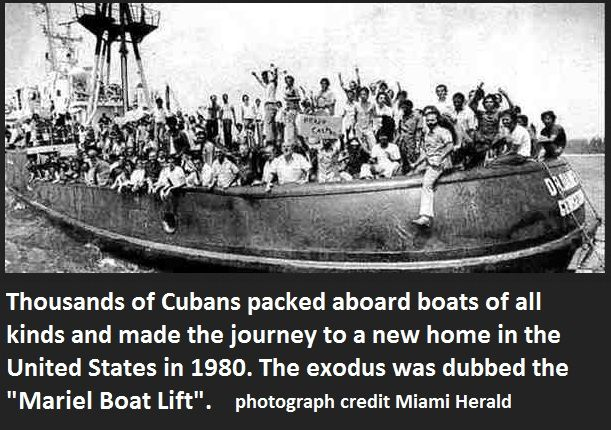
\includegraphics[width=\columnwidth]{fig/migration/mariel}
	\end{column}
\end{columns}

\end{frame}

\begin{frame}{ Russian Jews to Israel after 1989}

\begin{columns}[onlytextwidth]
	\begin{column}{0.4\textwidth}
		\begin{itemize}
			\item  the emigration of Russian Jews to Israel after 1989, when the Soviet Union relaxed its restrictions on such departures. 
			\item From late 1989 to 1996, some 670,000 Russian Jews
			emigrated to Israel, which increased the population in Israel by 11\% and its workforce by 14\%. 
			\item the Russian immigrants were more highly skilled than the existing Israeli population.
			\item 问题:这些高技能的犹太人当地工资水平会产生怎样的影响?
		\end{itemize}
	\end{column}
	\begin{column}{0.6\textwidth}
		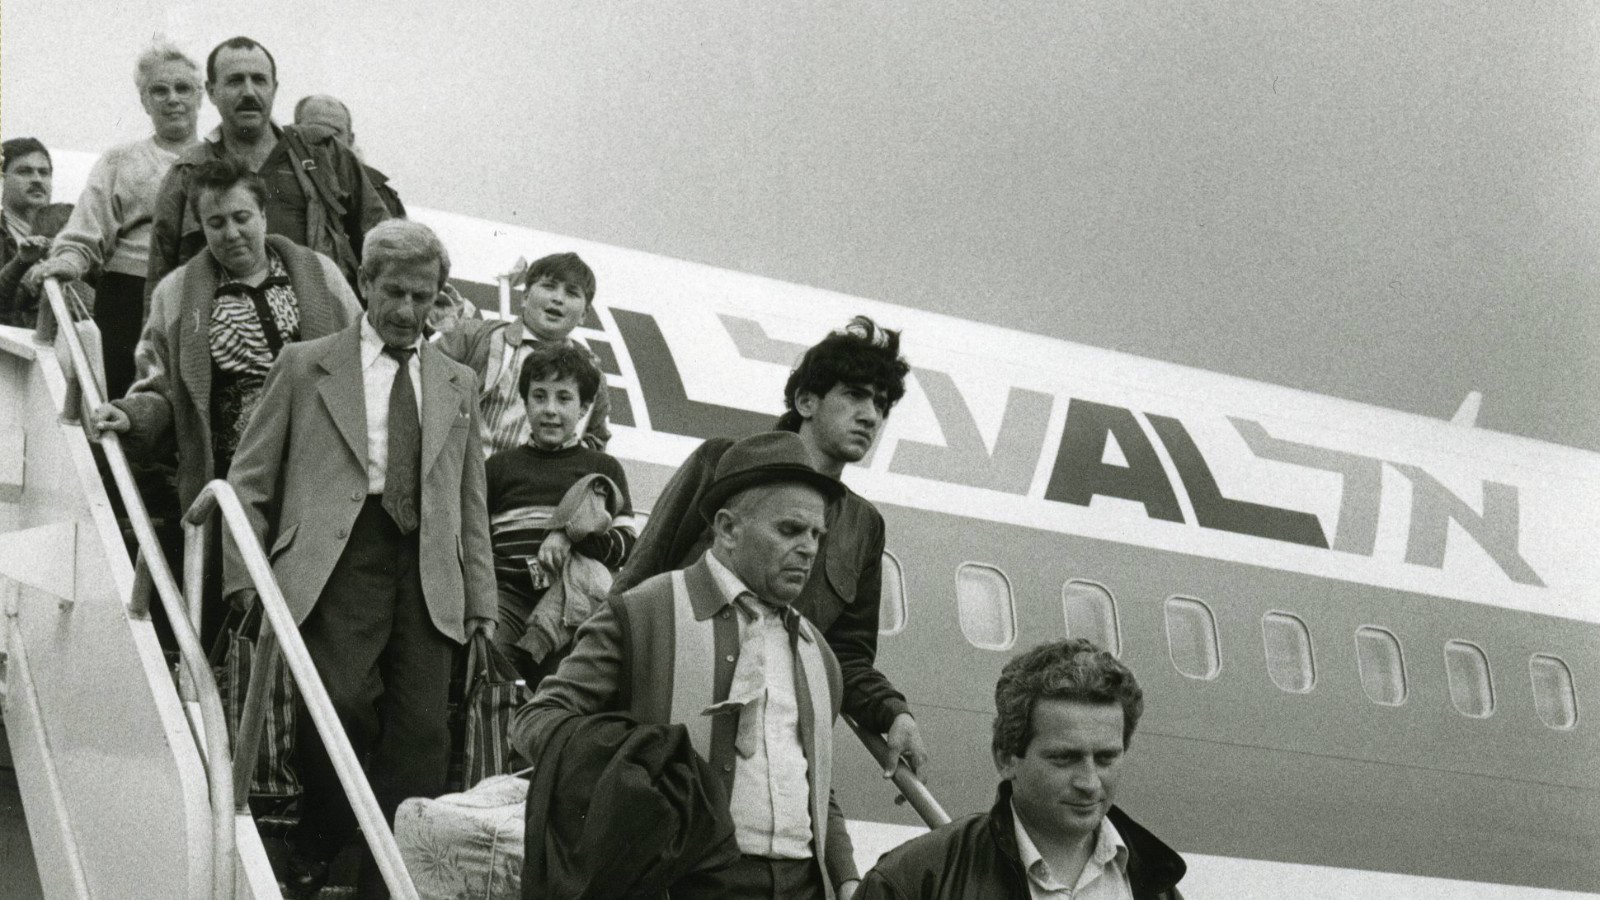
\includegraphics[width=\columnwidth]{fig/migration/israel}
	\end{column}
\end{columns}

\end{frame}

\begin{frame}{30年来有多少中国人移民美国-《2015胡润中国投资移民白皮书》}

\begin{columns}[onlytextwidth]
	\begin{column}{0.5\textwidth}
		\begin{itemize}
				\item  中国人海外移民最想去哪里? 
		\item 海外移民的主要Motivations
		\begin{itemize}
			\item 资产配置
			\item 分散风险
			\item 子女教育
		\end{itemize} 
		\item 220万中国出生者居住在美国
		\item 30年间160万人获得美国绿卡
		\item 中国人靠什么途径移民美国?
		  \begin{itemize}
		  	\item 直系亲属移民19.2\%。
		  	\item 非直系亲属移民34.1\%。
		  	\item 职业性移民25.3\% What's the meaning of \structure{Brain Drain}
		  	\item 通过庇护获得美国绿卡21\%
		  \end{itemize}	
		\end{itemize}
	\end{column}
	\begin{column}{0.5\textwidth}
		\begin{itemize}
			\item 华人在三大领域就业人数最多
			 \begin{enumerate}
			 	\item 管理和职业性领域53.4\%
			 	\item 销售和办公室文员领域20.8\%
			 	\item 服务业领域15.4\%
			 \end{enumerate}
		 \item 八成华裔移民属于工薪阶层
		\end{itemize}
	\end{column}
\end{columns}



\end{frame}

\section{Overview of Global Migration}

\begin{frame}{International migrants: numbers and trends}
\centering	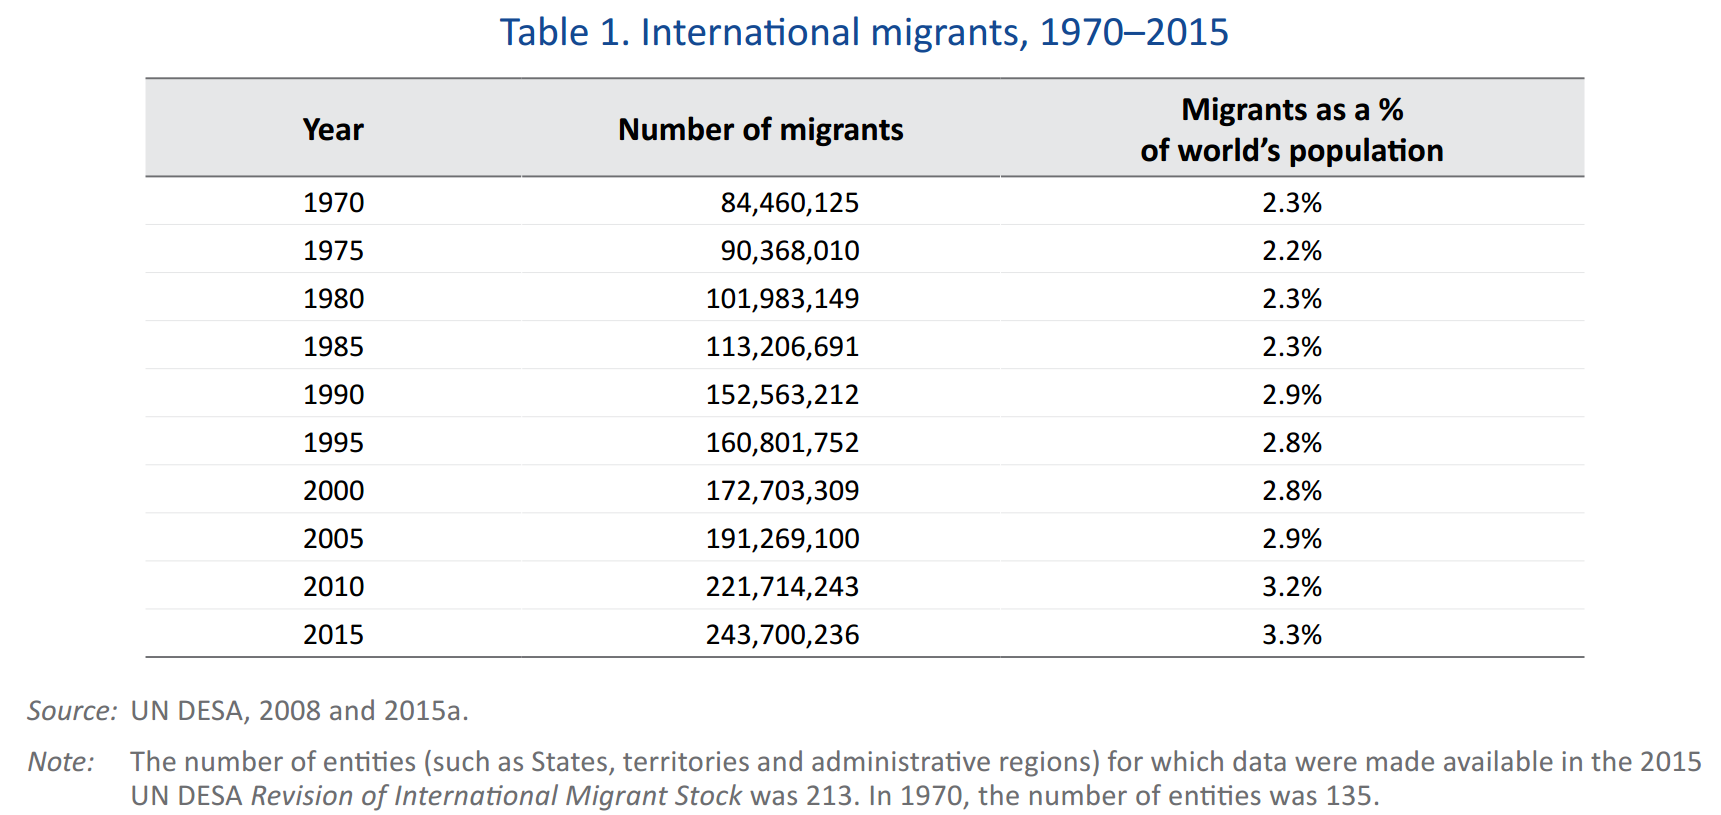
\includegraphics[width=\columnwidth]{fig/migration/mig1}
\end{frame}

\begin{frame}{proporton of internatonal migrants}
\centering 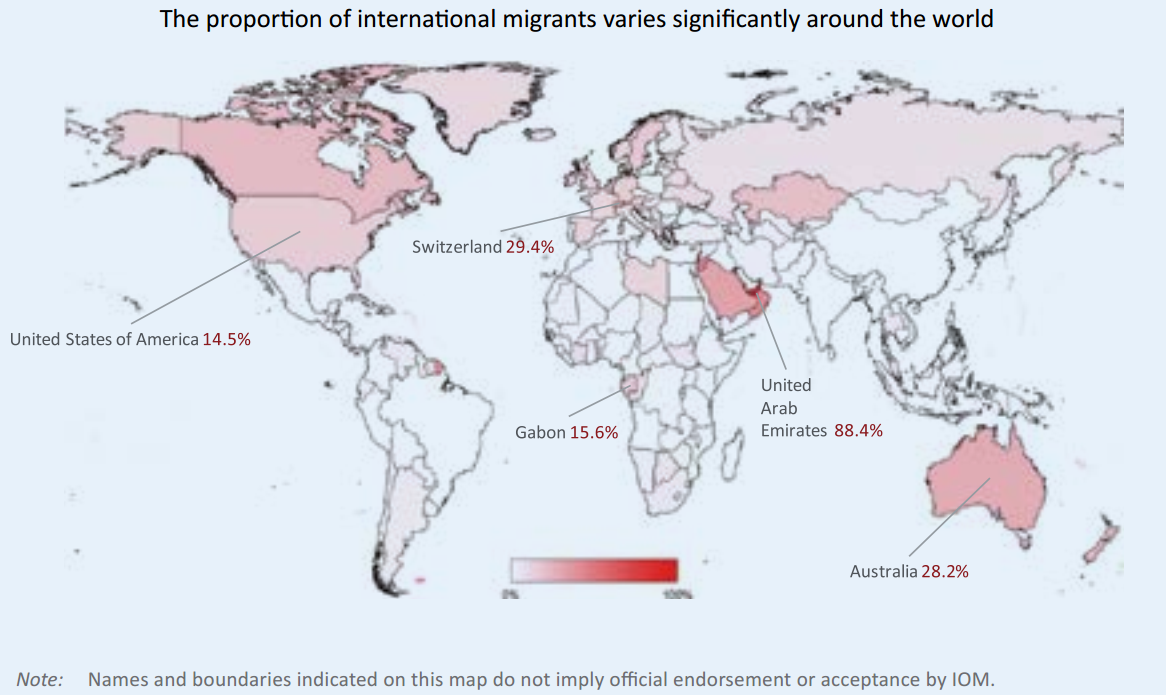
\includegraphics[width=0.8\columnwidth]{fig/migration/mig2}
\end{frame}

\begin{frame}{sexual structure of international migration}
\centering 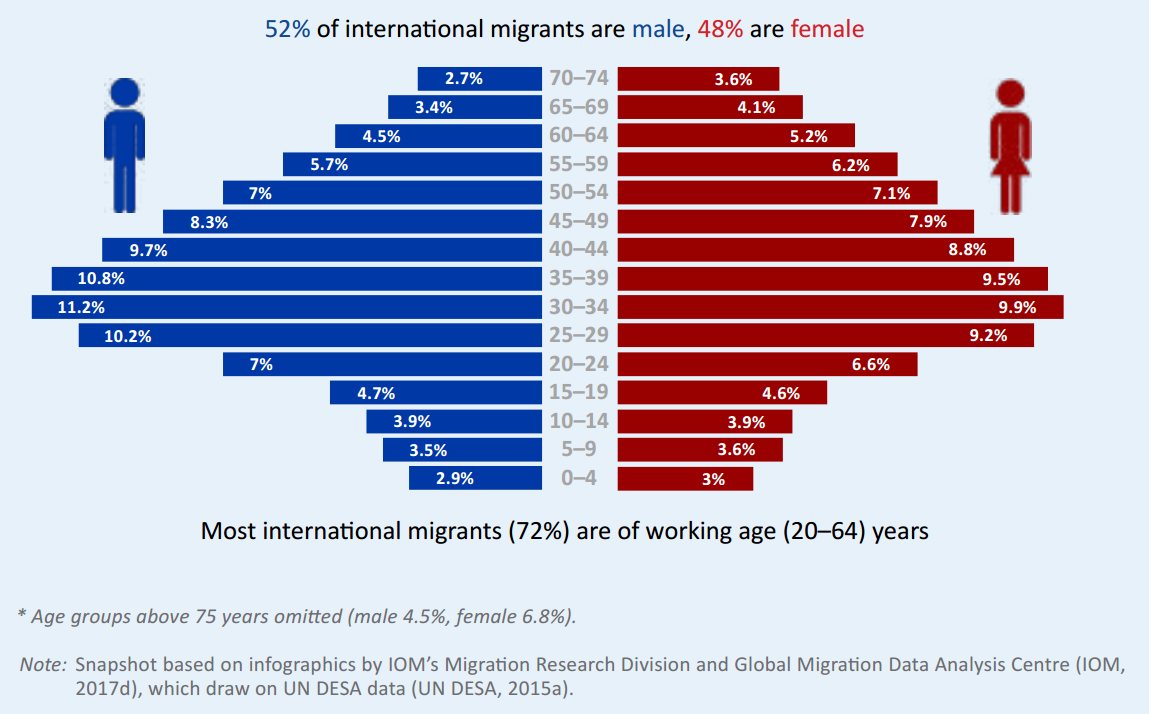
\includegraphics[width=0.8\columnwidth]{fig/migration/mig3}
\end{frame}

\begin{frame}{Main Destination and Main Origins}
\centering 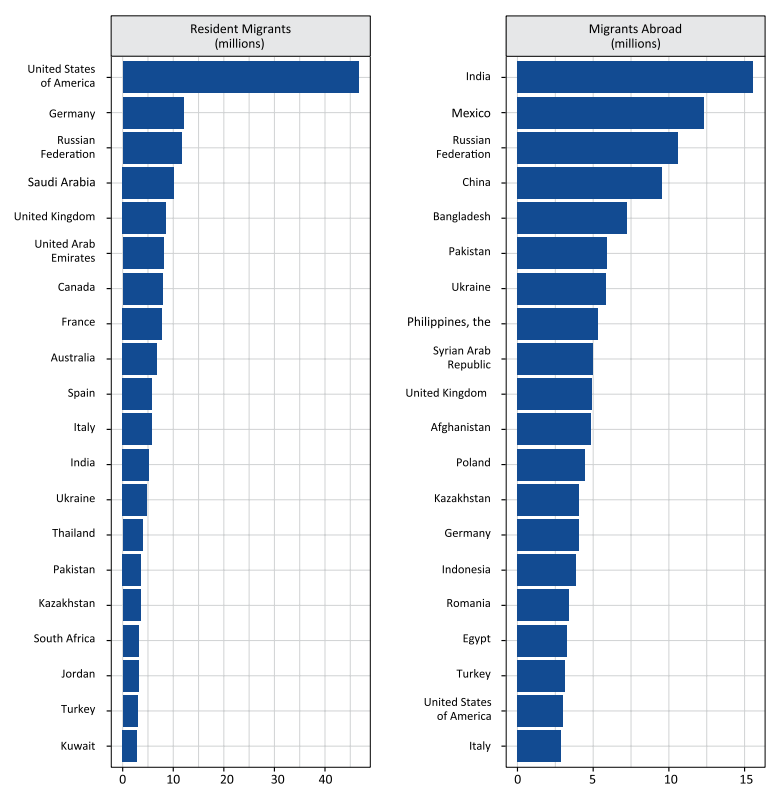
\includegraphics[width=0.6\columnwidth]{fig/migration/mig4}
\end{frame}

\begin{frame}{Refugees and asylum seekers}
  \begin{columns}
  	\begin{column}{0.5\textwidth}
  	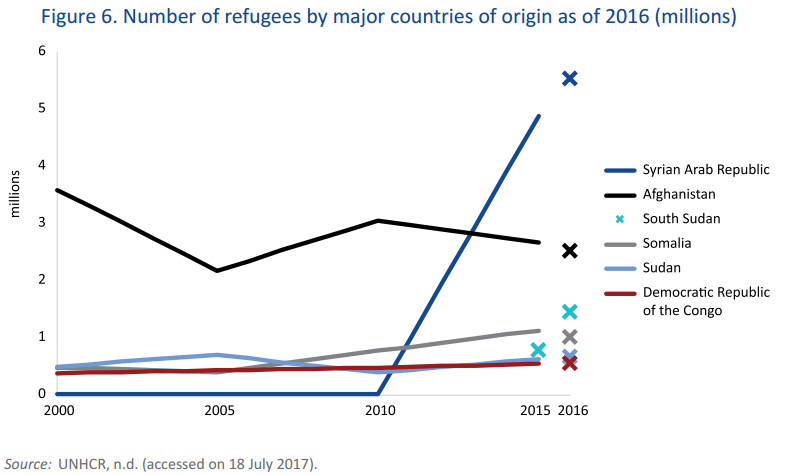
\includegraphics[width=\columnwidth]{fig/migration/mig5}
  \end{column}

  \begin{column}{0.5\textwidth}
  	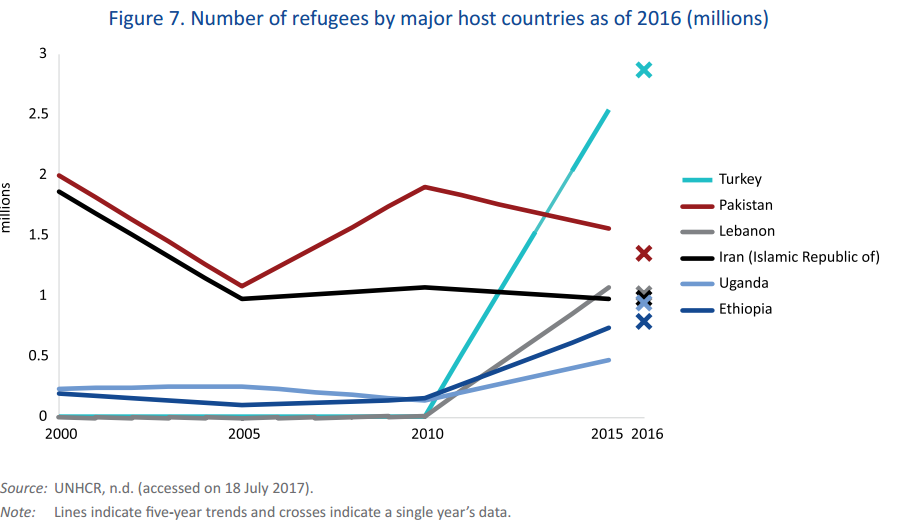
\includegraphics[width=\columnwidth]{fig/migration/mig6}
  \end{column}
  \end{columns}

\end{frame}

\section{An Application of the Specific Factors Model: Migration}
\begin{frame}{International Factor Movements }

\begin{itemize}
	\item Movements in factors of production include 
	
	\begin{itemize}
		\item labor migration (today) 
		\item the transfer of financial capital through international borrowing
		and lending (International Finace, another course I taught ) 
		\item transactions of multinational corporations involving direct ownership
		of foreign firms (the following sections) 
	\end{itemize}
	\item As we will see, the Specific Factors model is useful to conceptually
	analyze the causes and consequences of migration 
\end{itemize}
\end{frame}

\begin{frame}{A One-Good Model of Migration}

\begin{itemize}
\item Suppose there are two countries in the world, Home and Foreign 
\item They produce the same good, so there is no motive for trade in goods
in equilibrium 
\item This good is produced by combining land $T$ and labor $L$ using
a neoclassical production function $F(L,T)$ 
\item $F(L,T)$features constant returns to scale and diminishing marginal
products 
\item The supply of land in each country is fixed ($T$ and $T*$ ) 
\end{itemize}
\end{frame}

\begin{frame}{Real Wages }

\begin{itemize}
\item Real wages will be equal to the marginal product of labor in the production
of the good 
\[
w=\text{\ensuremath{\partial}}F(T,L)/\text{\ensuremath{\partial}}L
\]

\item Diminishing returns to scale imply that wages are decreasing in $L$ 
\item Complementarity between land and labor also implies that w is increasing
in $T$ 
\item Furthermore, $w>w*$ if and only if $T/L>T*/L*$ 
\end{itemize}
\end{frame}

\begin{frame}{Graphical Analysis }


\begin{columns}[onlytextwidth]
\begin{column}{0.4\textwidth}
\begin{itemize}
\item The total wage bill is given by $w\cdot L$ 
\item The remaining output (i.e., income) accrues to land -owners in the
form of land rents 
\item In the figure this is the area below the MPL curve and above the real
wage level
\end{itemize}

\end{column}
\begin{column}{0.6\textwidth}
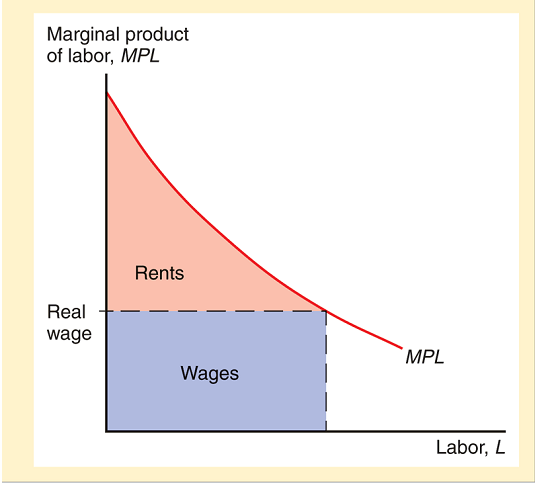
\includegraphics[width=0.8\columnwidth]{fig/migration/lec4-27}
\end{column}
\end{columns}

\end{frame}

\begin{frame}{Incentives for Migration}


\begin{columns}[onlytextwidth]
\begin{column}{0.4\textwidth}
\begin{itemize}
\item A land-abundant country (say Home) has a higher wage without migration 
\item Hence, workers might have an incentive to migrate from Foreign to
Home 
\item More generally, workers have an incentive to migrate away from countries
where they are \textbf{\textcolor{blue}{relatively abundant }}
\end{itemize}

\end{column}
\begin{column}{0.6\textwidth}
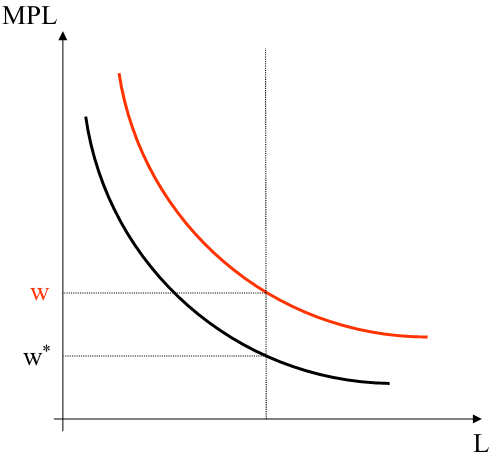
\includegraphics[width=0.8\columnwidth]{fig/migration/lec4-28}
\end{column}
\end{columns}

\end{frame}

\begin{frame}{Level of Migration }


\begin{columns}[onlytextwidth]
\begin{column}{0.4\textwidth}
\begin{itemize}
\item How much immigration will there be? 
\item Note that as $L$ at Home increases, $w$ falls, while as $L*$ in
Foreign falls, $w*$ increases 
\item We can just flip around the Foreign $MPL$ schedule 
\item Migration from Foreign to Home is $L_{2}-L_{1}$
\end{itemize}

\end{column}
\begin{column}{0.6\textwidth}
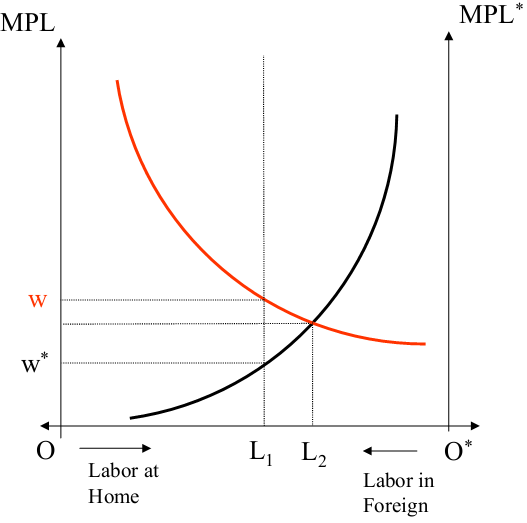
\includegraphics[width=0.8\columnwidth]{fig/migration/lec4-29}
\end{column}
\end{columns}

\end{frame}

\begin{frame}{Effect of Migration on Output }


\begin{columns}[onlytextwidth]
\begin{column}{0.4\textwidth}
\begin{itemize}
\item Note that output in each country is equal to the area below the MPL
curve up to the level of employment 
\item Relative to the equilibrium in $L_{1}$ , the area in blue below the
$MPL^{*}$ between $L_{1}$ and $L_{2}$ is lost 
\item But this is gained at Home, as well as the extra area in green 
\item So world output goes up! 
\end{itemize}

\end{column}
\begin{column}{0.6\textwidth}
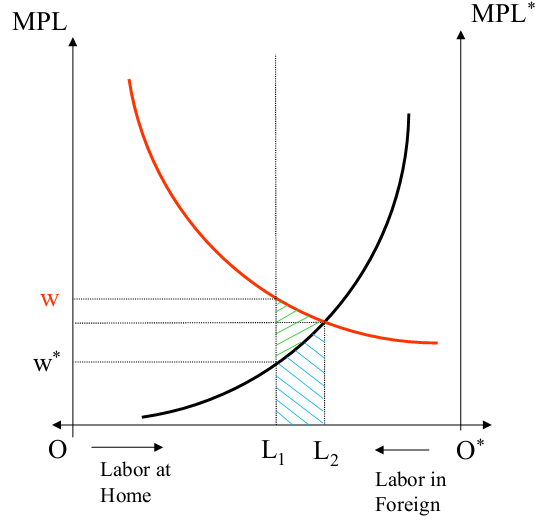
\includegraphics[width=0.8\columnwidth]{fig/migration/lec4-30}
\end{column}
\end{columns}

\end{frame}

\begin{frame}{Distributional Effects}

\begin{itemize}
\item Notice however that not everybody gains from migration 
\item Native workers in the labor - scarce country are worse off 
\item Landowners in the labor - abundant country are also worse off 
\item But these agents could (theoretically) be compensated so as to make
migration Pareto superior
\end{itemize}
\end{frame}

\begin{frame}{Some Caveats }

\begin{itemize}
\item Although it seems intuitive that immigration will hurt native workers
\item If the second factor is “skilled workers” rather than “land”, then
these skilled workers in the recipient country will benefit from migration 
\item In the Heckscher - Ohlin model studied in the last lectures,
wages might actually be predicted to show little sensitivity to migration 
\end{itemize}
\end{frame}

\begin{frame}{Impediments to Migration }

\begin{itemize}
\item In the real world, wages do not actually equalize due to several factors

\begin{itemize}
\item barriers to migration such as policies restricting immigration 
\item differences in skill (perhaps due to language) 
\item natural reluctance to move 
\end{itemize}
\end{itemize}
\end{frame}

\begin{frame}{Empirical Evidence}

\begin{itemize}
\item Early migration wave: from low wage to high wage 
\item Wages subsequently grew faster in origin countries
\begin{figure}


\begin{centering}
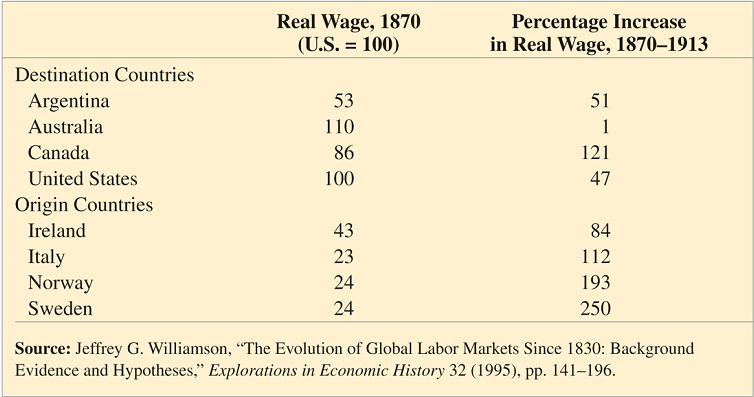
\includegraphics[width=10cm]{fig/migration/lec4-31}
\par\end{centering}

\end{figure}

\end{itemize}
\end{frame}

\begin{frame}{U.S. Immigration }

\begin{itemize}
\item Two waves of immigration: early 20 th cent. (Eastern \& Southern Europe)
and last few decades (Central/South America and Asia) 
\begin{figure}


\begin{centering}
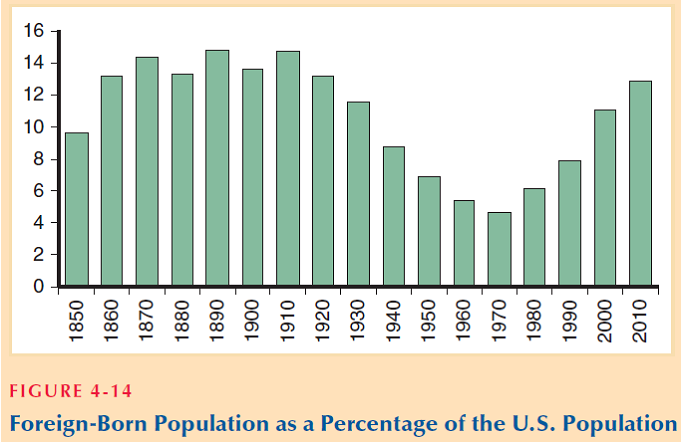
\includegraphics[width=9cm]{fig/migration/lec4-32}
\par\end{centering}

\end{figure}

\end{itemize}
\end{frame}

\begin{frame}{Recent U.S. Immigration }

\begin{itemize}
\item Recent growth especially high among workers with the lowest education
levels and the highest education levels
\begin{figure}


\begin{centering}
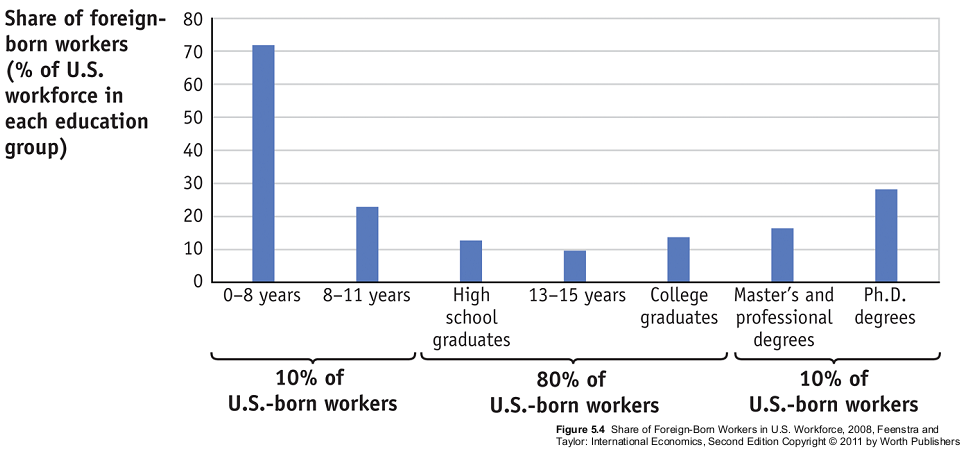
\includegraphics[width=11cm]{fig/migration/lec4-33}
\par\end{centering}

\end{figure}

\end{itemize}
\end{frame}

\begin{frame}{Borjas, Freeman and Katz (1996) }

\begin{itemize}
\item BFK use variation across U.S. regions in the distribution of the immigrant
population to analyze the effect of immigration on wages 
\item For 1980 and 1990, they estimate separately for men and for women
the equation: 
\[
lnw_{ijk}=\alpha_{t}AGE_{i}+\beta_{t}EDUC_{i}+\gamma_{t}(I/N){}_{jk}+e_{ijk}
\]

\item $i$ is individual,$j$ is education group and $k$ is region 
\item $I/N$ is the ratio of immigrants to natives in the relevant region
and education category 
\end{itemize}
\end{frame}

\begin{frame}{BFK (1996)}


\begin{columns}[onlytextwidth]
\begin{column}{0.5\textwidth}
\begin{itemize}
\item They find that the coefficient γ is not robust (sometimes +, sometimes
−) 
\item \textbf{\textcolor{blue}{Problem of selection}} : do immigrants choose
to move to regions with high wages, and are people with skills in
high demand more likely to migrate? 
\item When regressing changes in wages on regional changes in I/N, they
find generally (though not always) negative coefficients 
\end{itemize}

\end{column}
\begin{column}{0.5\textwidth}
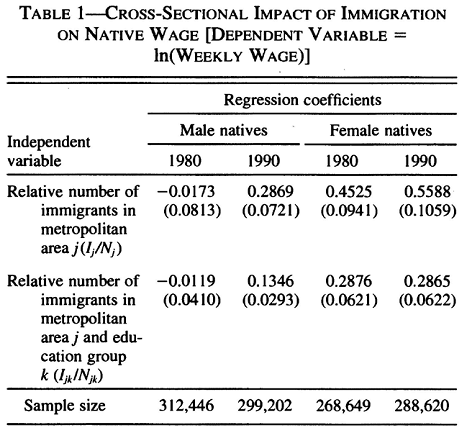
\includegraphics[width=\columnwidth]{fig/migration/lec4-34}
\end{column}
\end{columns}

\end{frame}

\begin{frame}{A Natural Experiment: Mariel Boatlift}


\begin{columns}[onlytextwidth]
\begin{column}{0.3\textwidth}
\begin{itemize}
\item Mass movement of 125,000 Cubans who departed from Cuba’s Mariel harbor
for the United States between April 15 and October 31, 1980
\end{itemize}

\end{column}
\begin{column}{0.7\textwidth}
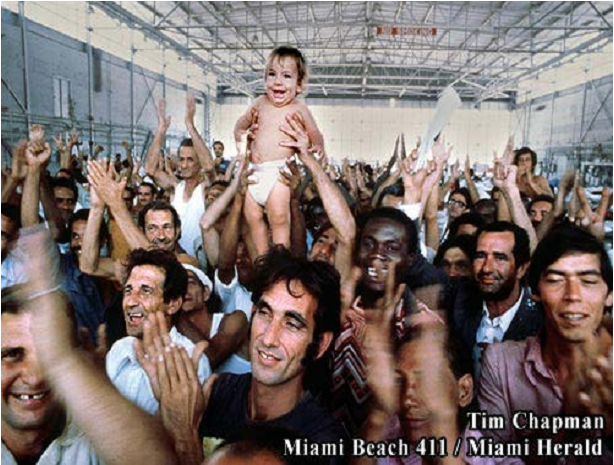
\includegraphics[width=0.9\columnwidth]{fig/migration/lec4-35}
\end{column}
\end{columns}

\end{frame}

\begin{frame}{A Natural Experiment }

\begin{itemize}
\item Most Cubans ended up in Miami (increased Miami labor force by 7\%) 
\item Empirical strategy (Card, 1990): how did the inflow affect Miami wages
and employment relative to \textbf{\textcolor{blue}{comparable}} cities
(Atlanta, Houston, Los Angeles, Tampa)? 
\item Answer: virtually no effect 
\item Concerns about whether Cuban immigrants were “representative” of typical
immigrants
\end{itemize}
\end{frame}

\begin{frame}{The Bigger Picture}

\begin{itemize}
\item Of course, even when only focusing on economic considerations, the
case for immigration needs to take other factors into account 

\begin{itemize}
\item For instance, effects on tax revenue and government spending 
\end{itemize}
\item Swiss author Max Frisch: “\textbf{\textcolor{blue}{We asked for labor,
but people came}}” 
\end{itemize}
\end{frame}





\end{document}
